%
% parabolic.tex -- characteristics and parabolic PDE
%
% (c) 2019 Prof Dr Andreas Müller, Hochschule Rapperswil
%
\documentclass[tikz,12pt]{standalone}
\usepackage{amsmath}
\usepackage{times}
\usepackage{txfonts}
\usepackage{pgfplots}
\usepackage{csvsimple}
\usetikzlibrary{arrows,intersections,math}
\begin{document}
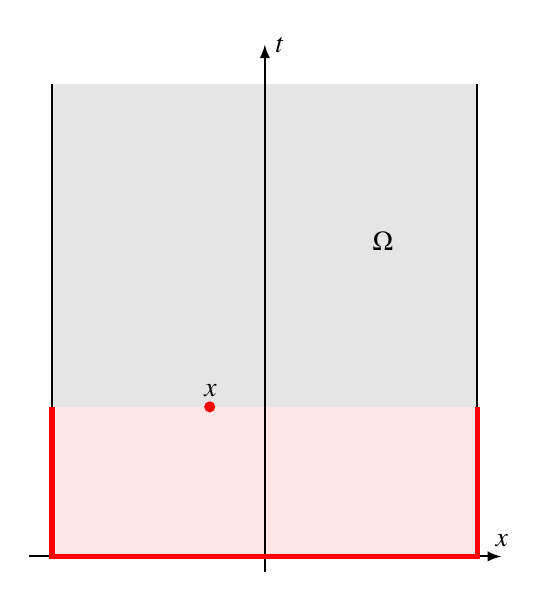
\begin{tikzpicture}[>=latex]

\def\radius{2.7}
\def\h{1.9}

\fill[color=gray!20] (-\radius,0)--(\radius,0)--(\radius,6)--(-\radius,6)--cycle;
\fill[color=red!10] (-\radius,0)--(\radius,0)--(\radius,\h)--(-\radius,\h)--cycle;
\draw[line width=0.7pt] (-\radius,0)--(-\radius,6);
\draw[line width=0.7pt] (\radius,0)--(\radius,6);

\draw[->,line width=0.7pt] (-3,0)--(3,0) coordinate[label={$x$}];
\draw[->,line width=0.7pt] (0,-0.2)--(0,6.5) coordinate[label={right:$t$}];

\draw[line width=2pt,color=red] (-\radius,\h)--(-\radius,0)--(\radius,0)--(\radius,\h);

\fill[color=red] (-0.7,\h) circle[radius=2pt];
\node at (-0.7,\h) [above] {$x$};

\node at (1.5,4) {$\Omega$};

\end{tikzpicture}
\end{document}

